\chapter{Bayesian Causal Inference Model Estimates} 
\label{App-bci-plots} 
\lhead{Appendix C. \emph{Bayesian Causal Inference Model Estimates}} 

The plots in this appendix show the predictions of proximal hand's inferred positions according to the Bayesian Causal Inference Model, along with the estimated target locations (measured experimentally) for different target locations.

The red line indicates position of the visual signal of the proximal hand, while the blue line indicates the position of the proprioceptive signal, that is, the location of the placement of the real hand. The black curve indicates the probability density function denoting the probability of the location of the hand, after multi-sensory integration process postulated by the Bayesian Causal Inference Model. The mode of the distribution indicates the inferred position of the hand. The green dotted line indicates the veridical position of the reach target, while the solid green line indicates the (average) located estimated by the subjects. The yellow line indicates the initial position of the action hand. Panels A to E are ordered by the increasing proximity of the inferred hand position to the reach target.


\begin{figure}[h]
\centering       
    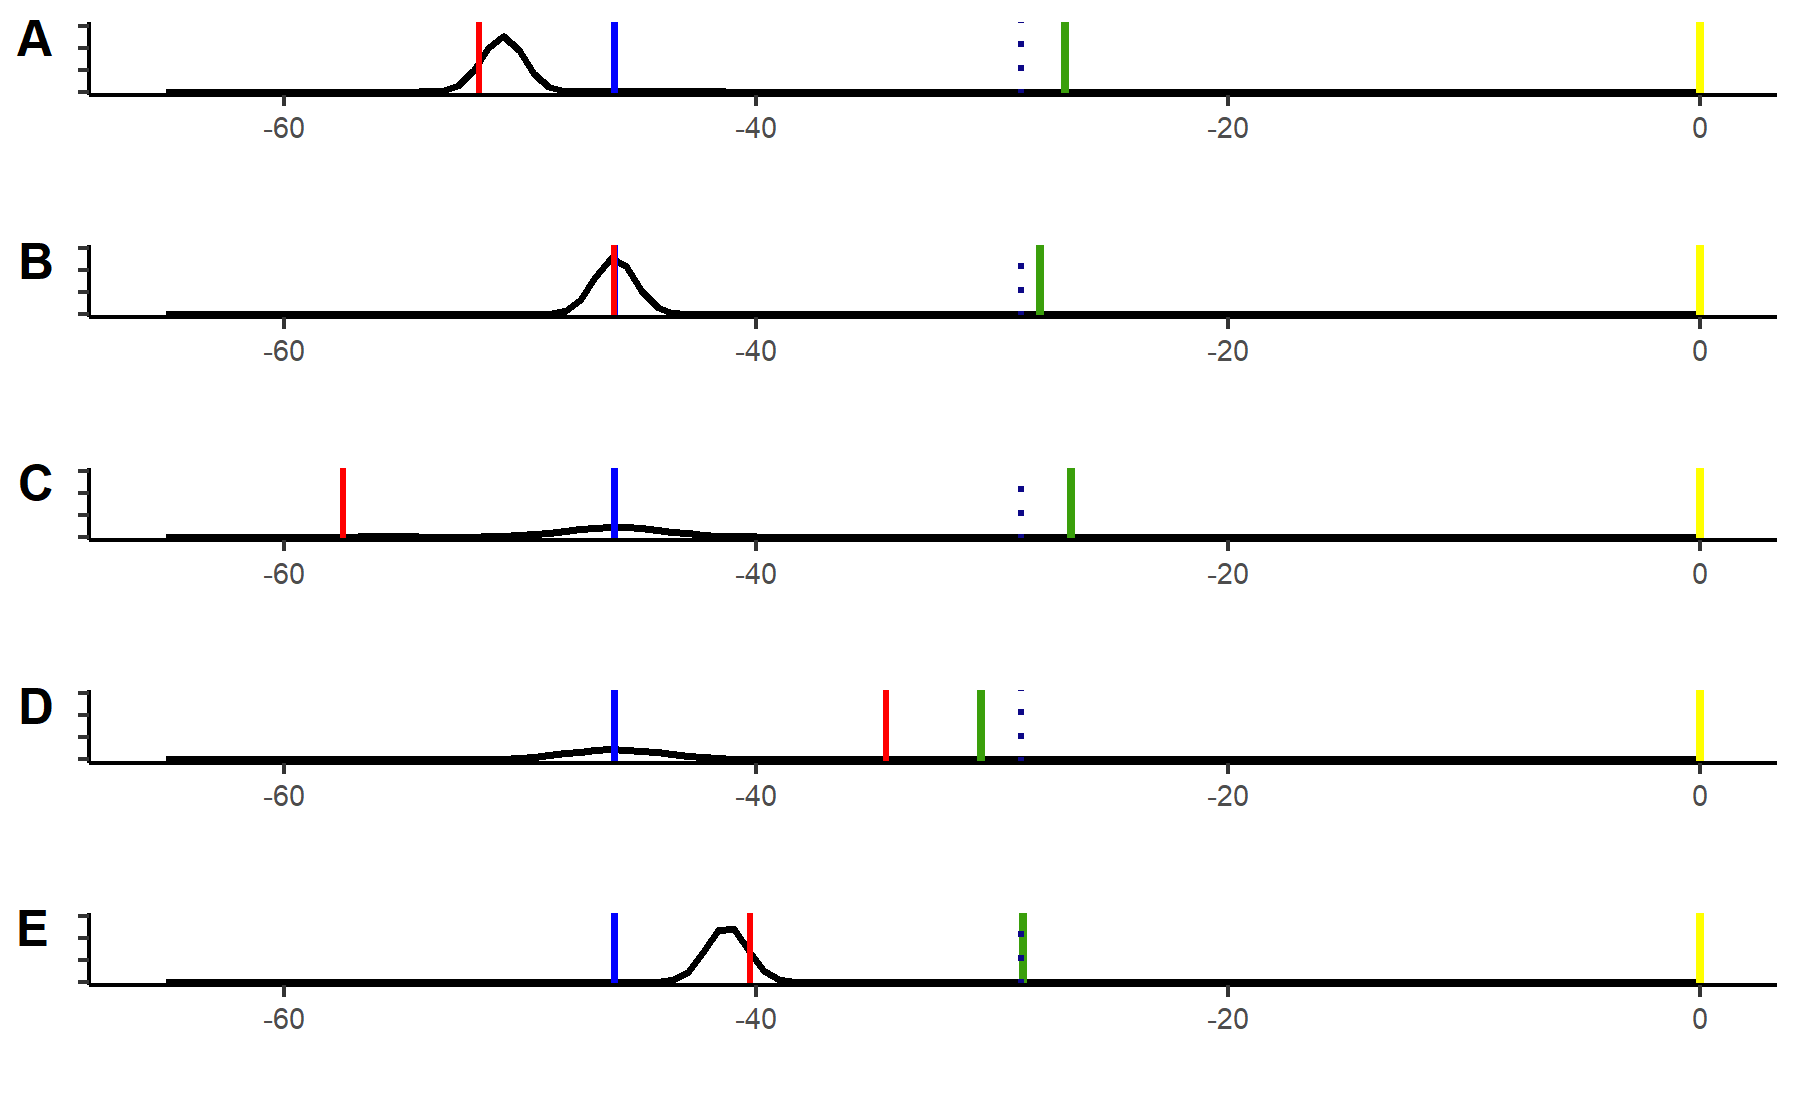
\includegraphics[width=\textwidth, keepaspectratio]{Images/bci-plots/bci_plot17-25.png}
    \caption{Target Location = 28.75 cm}
    \label{}
\end{figure}

\begin{figure}[h]
\centering       
    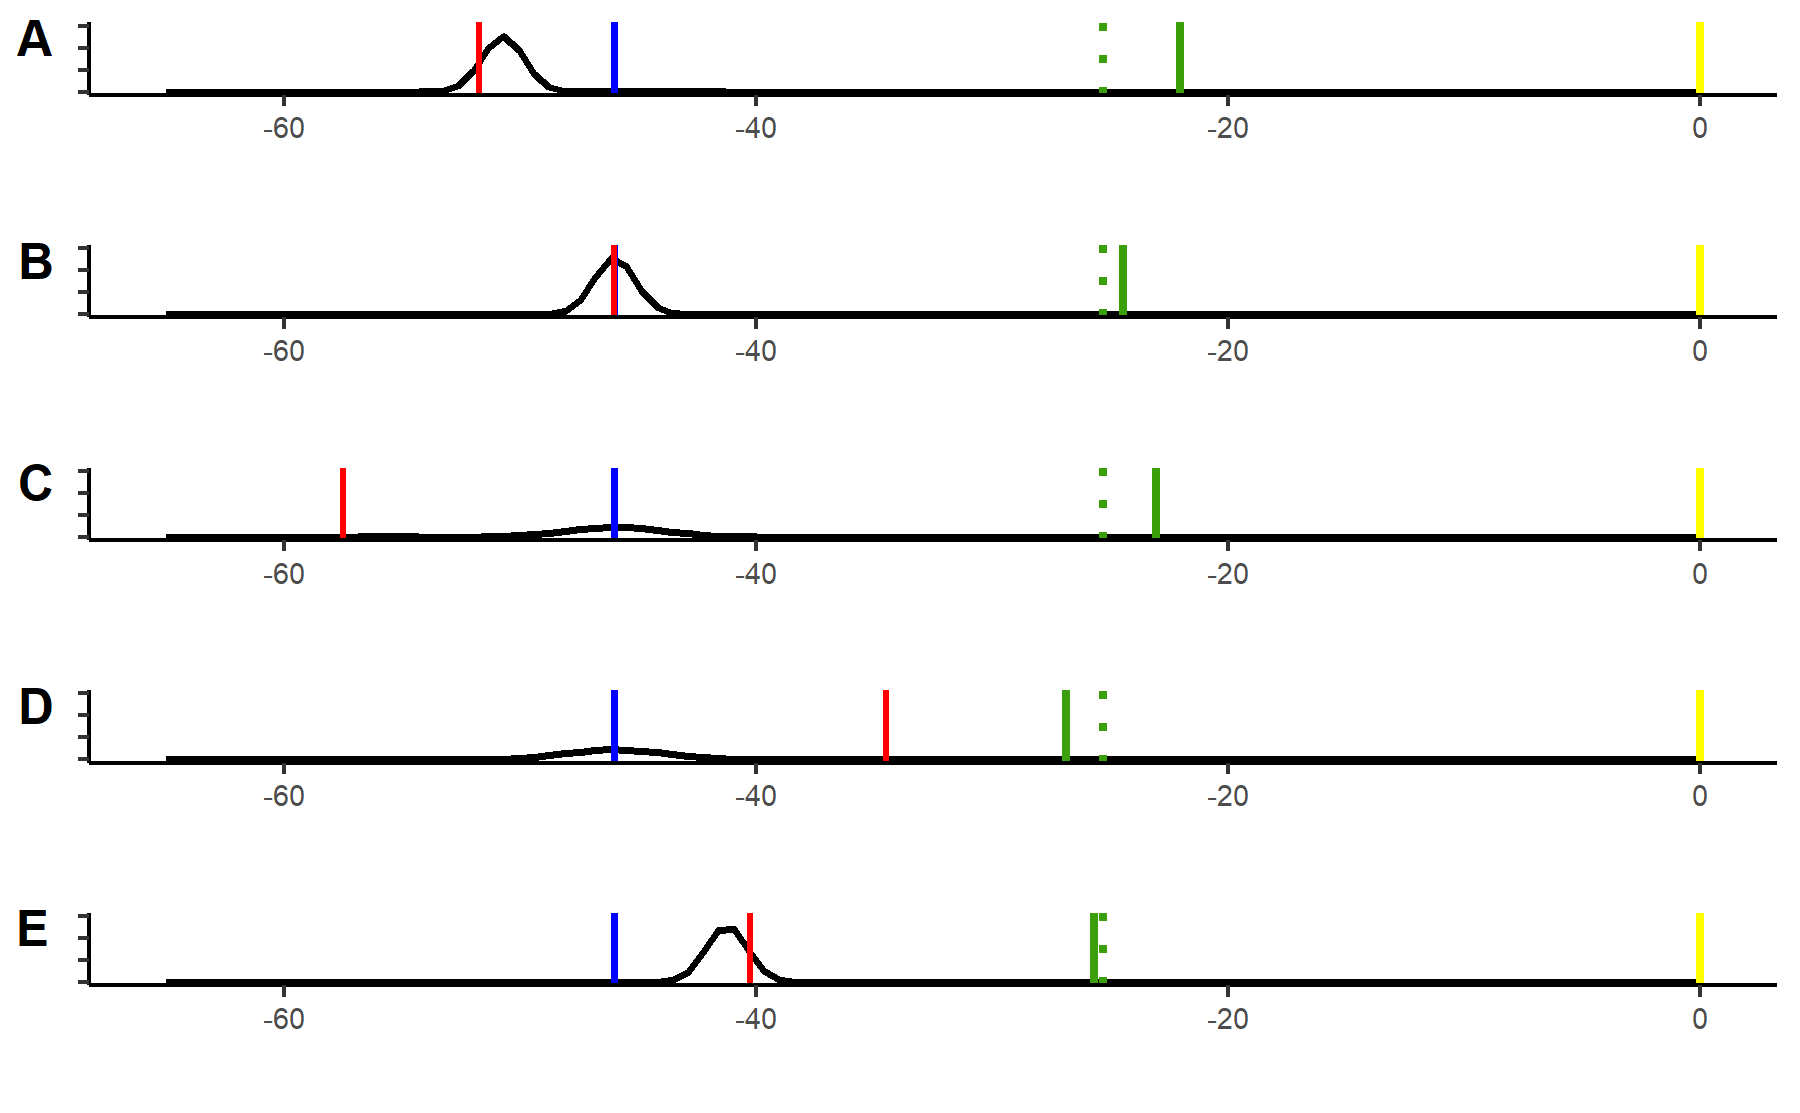
\includegraphics[width=\textwidth, keepaspectratio]{Images/bci-plots/bci_plot20-7.png}
    \caption{Target Location = 25.3 cm}
    \label{}
\end{figure}

\begin{figure}[h]
\centering       
    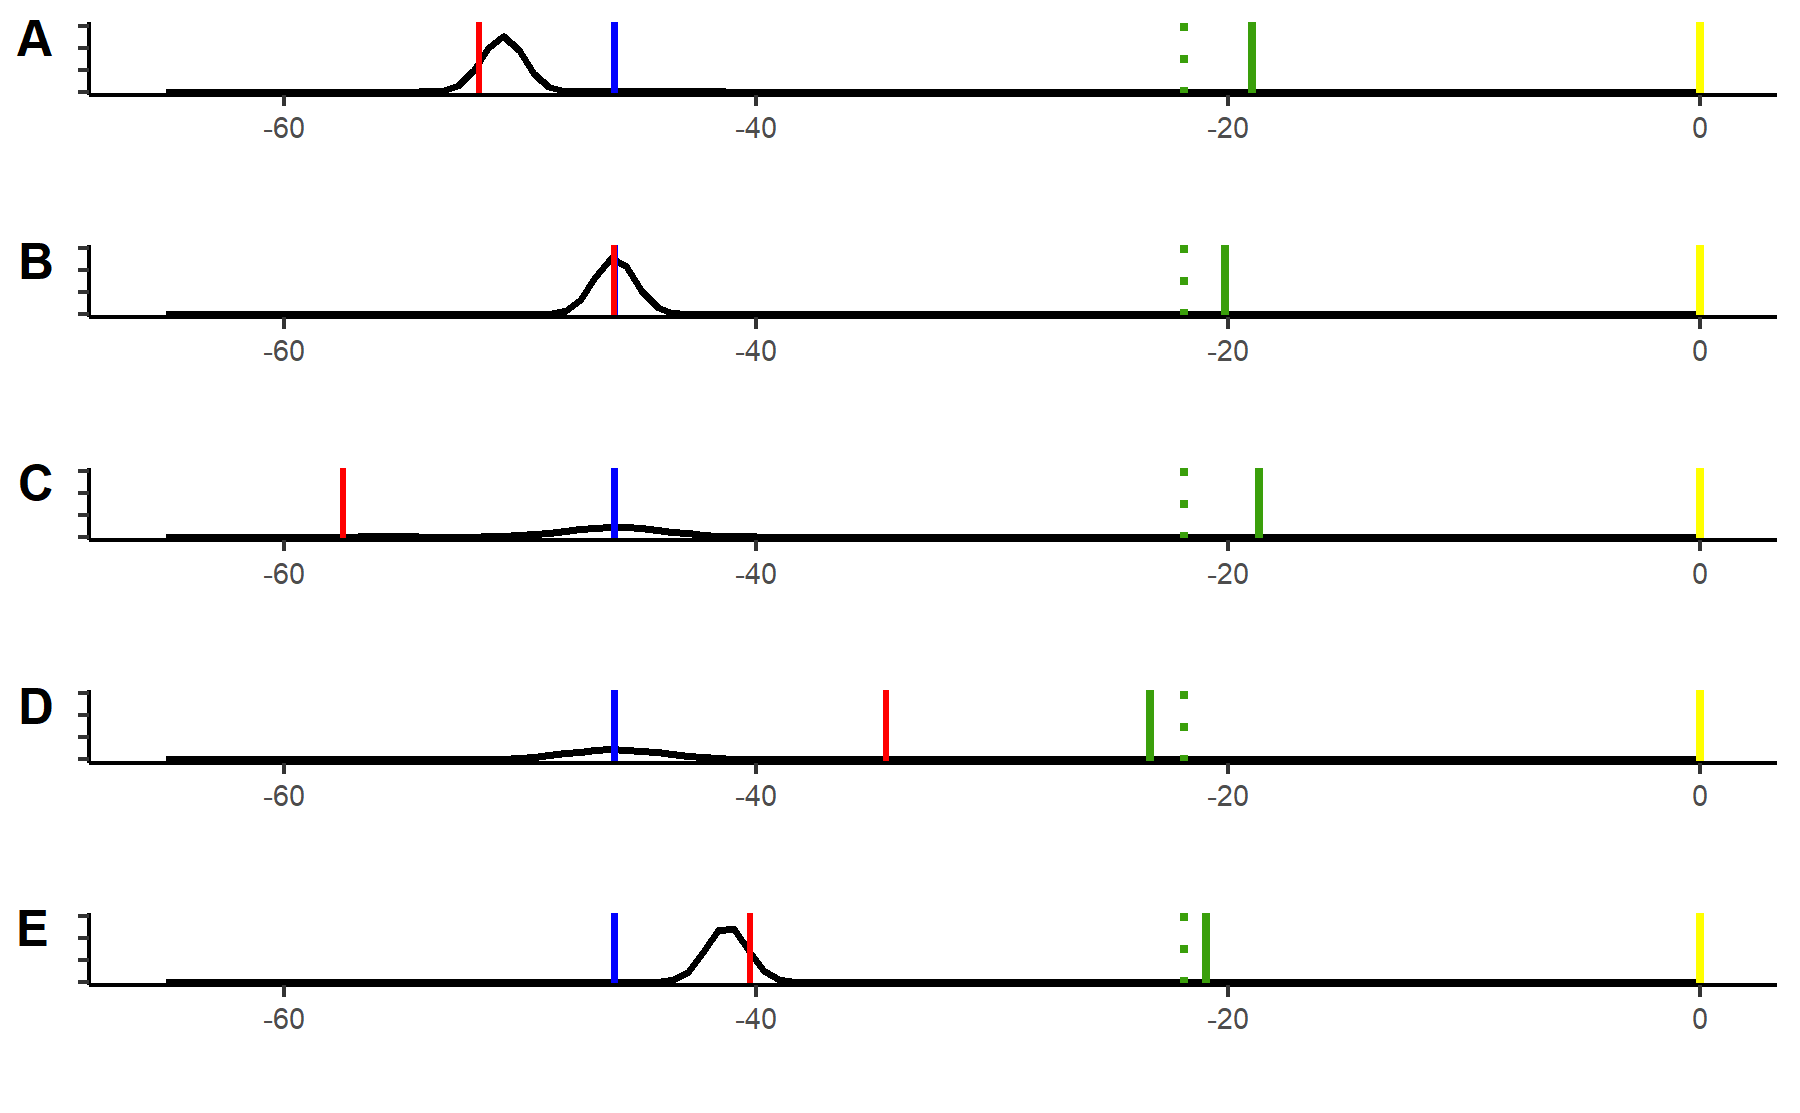
\includegraphics[width=\textwidth, keepaspectratio]{Images/bci-plots/bci_plot24-15.png}
    \caption{Target Location = 21.85 cm}
    \label{}
\end{figure}

\begin{figure}[h]
\centering       
    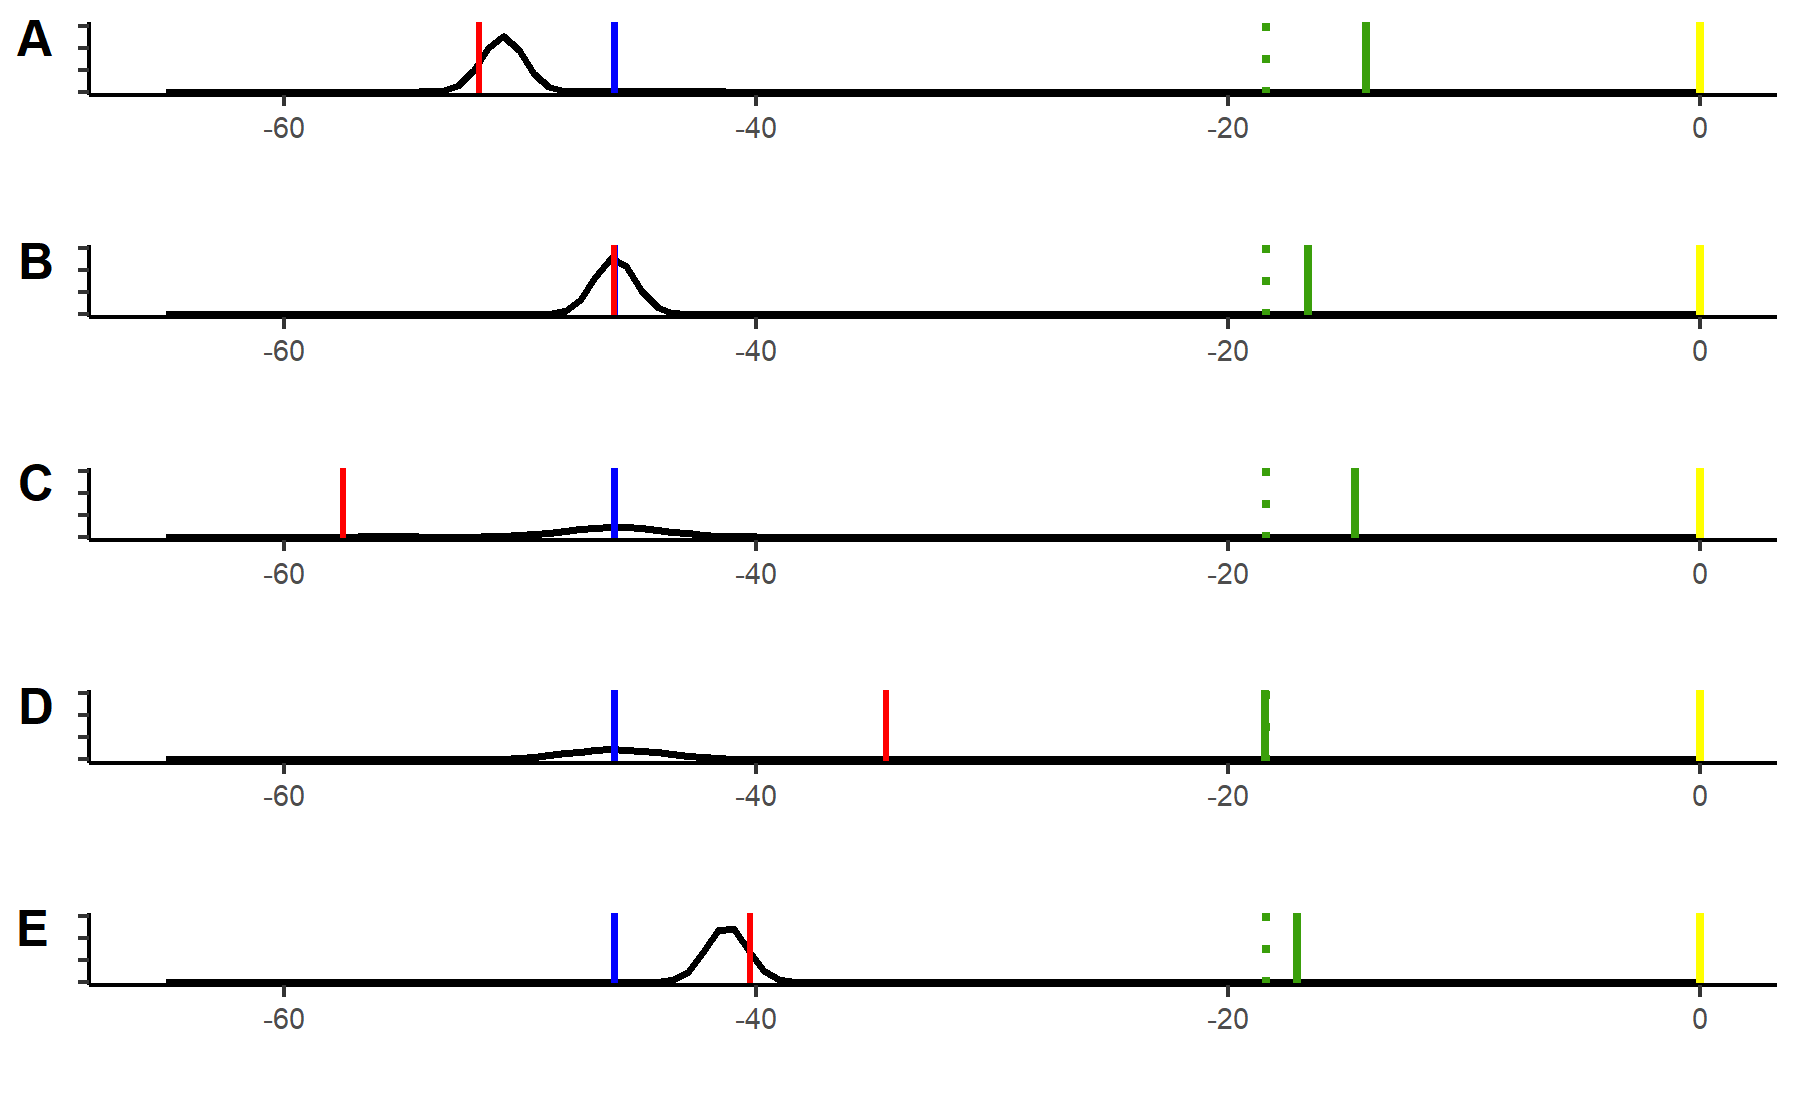
\includegraphics[width=\textwidth, keepaspectratio]{Images/bci-plots/bci_plot27.6.png}
    \caption{Target Location = 18.4 cm}
    \label{}
\end{figure}

\begin{figure}[h]
\centering       
    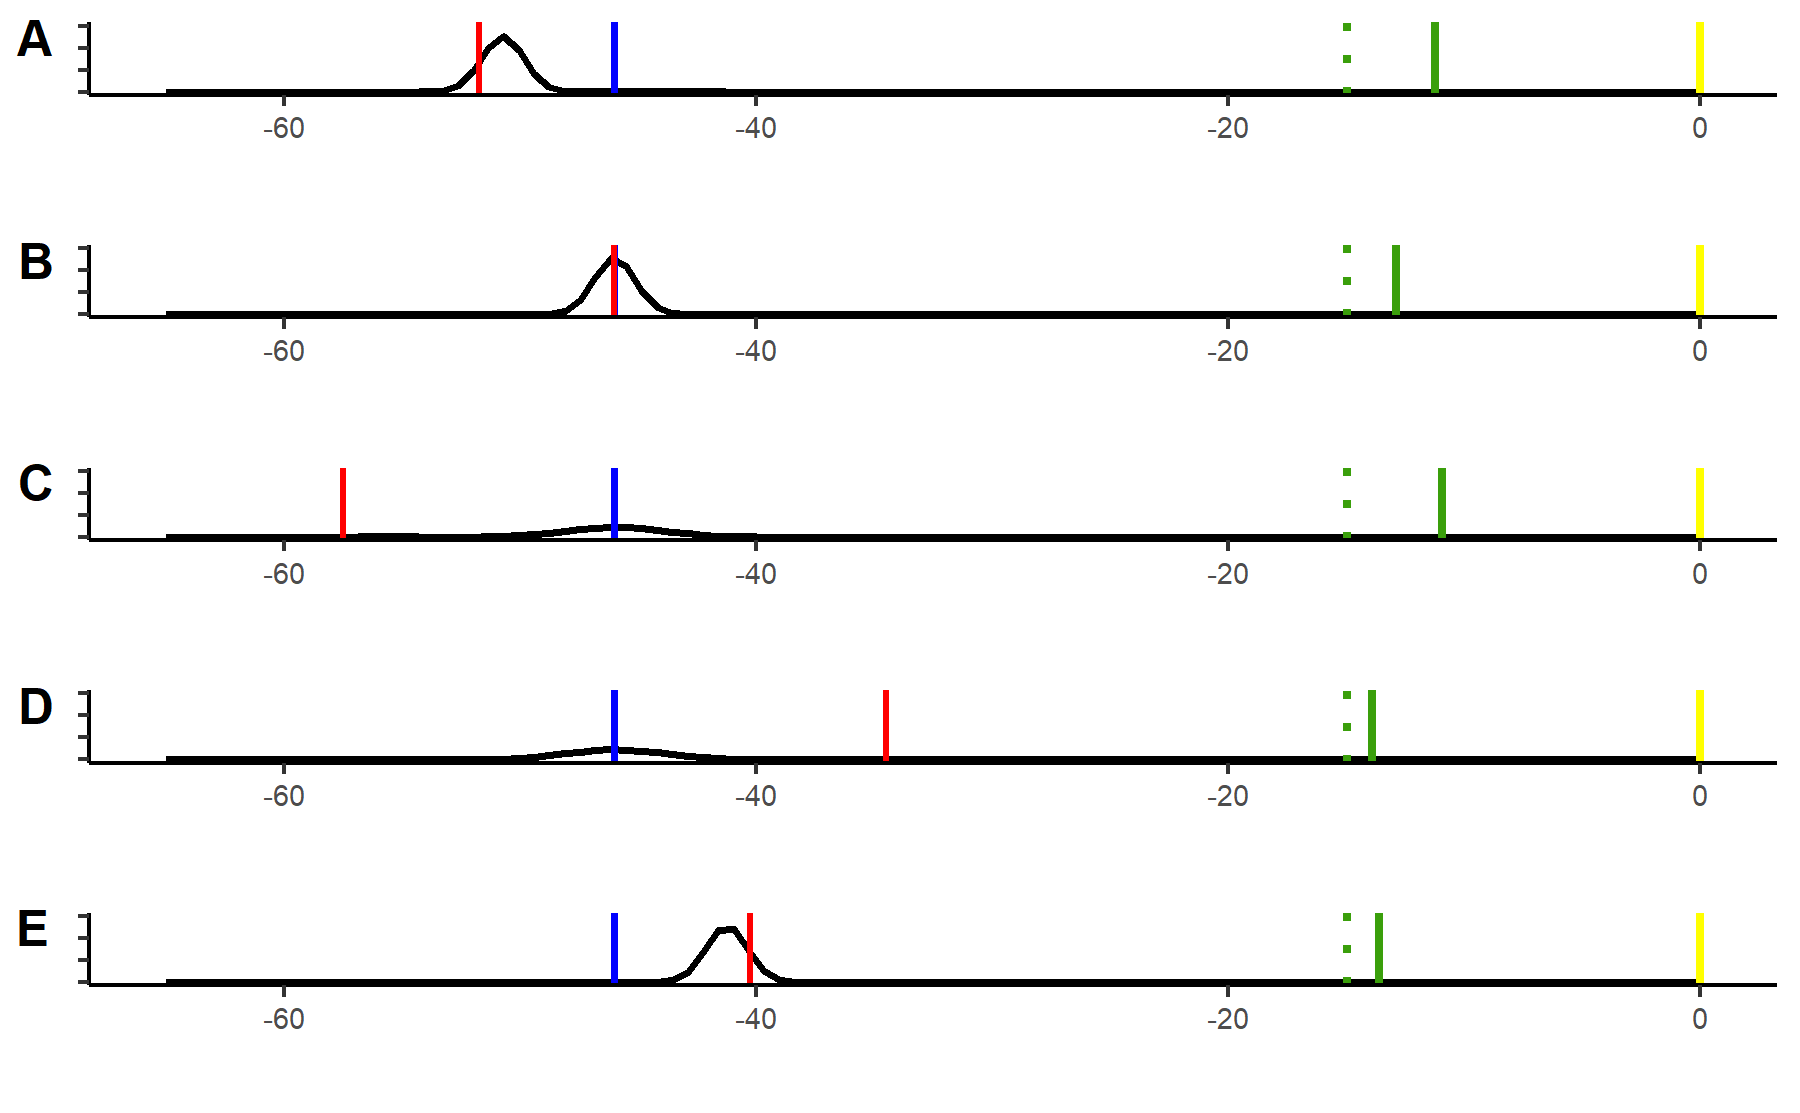
\includegraphics[width=\textwidth, keepaspectratio]{Images/bci-plots/bci_plot31-05.png}
    \caption{Target Location = 14.95 cm}
    \label{}
\end{figure}

\begin{figure}[h]
\centering       
    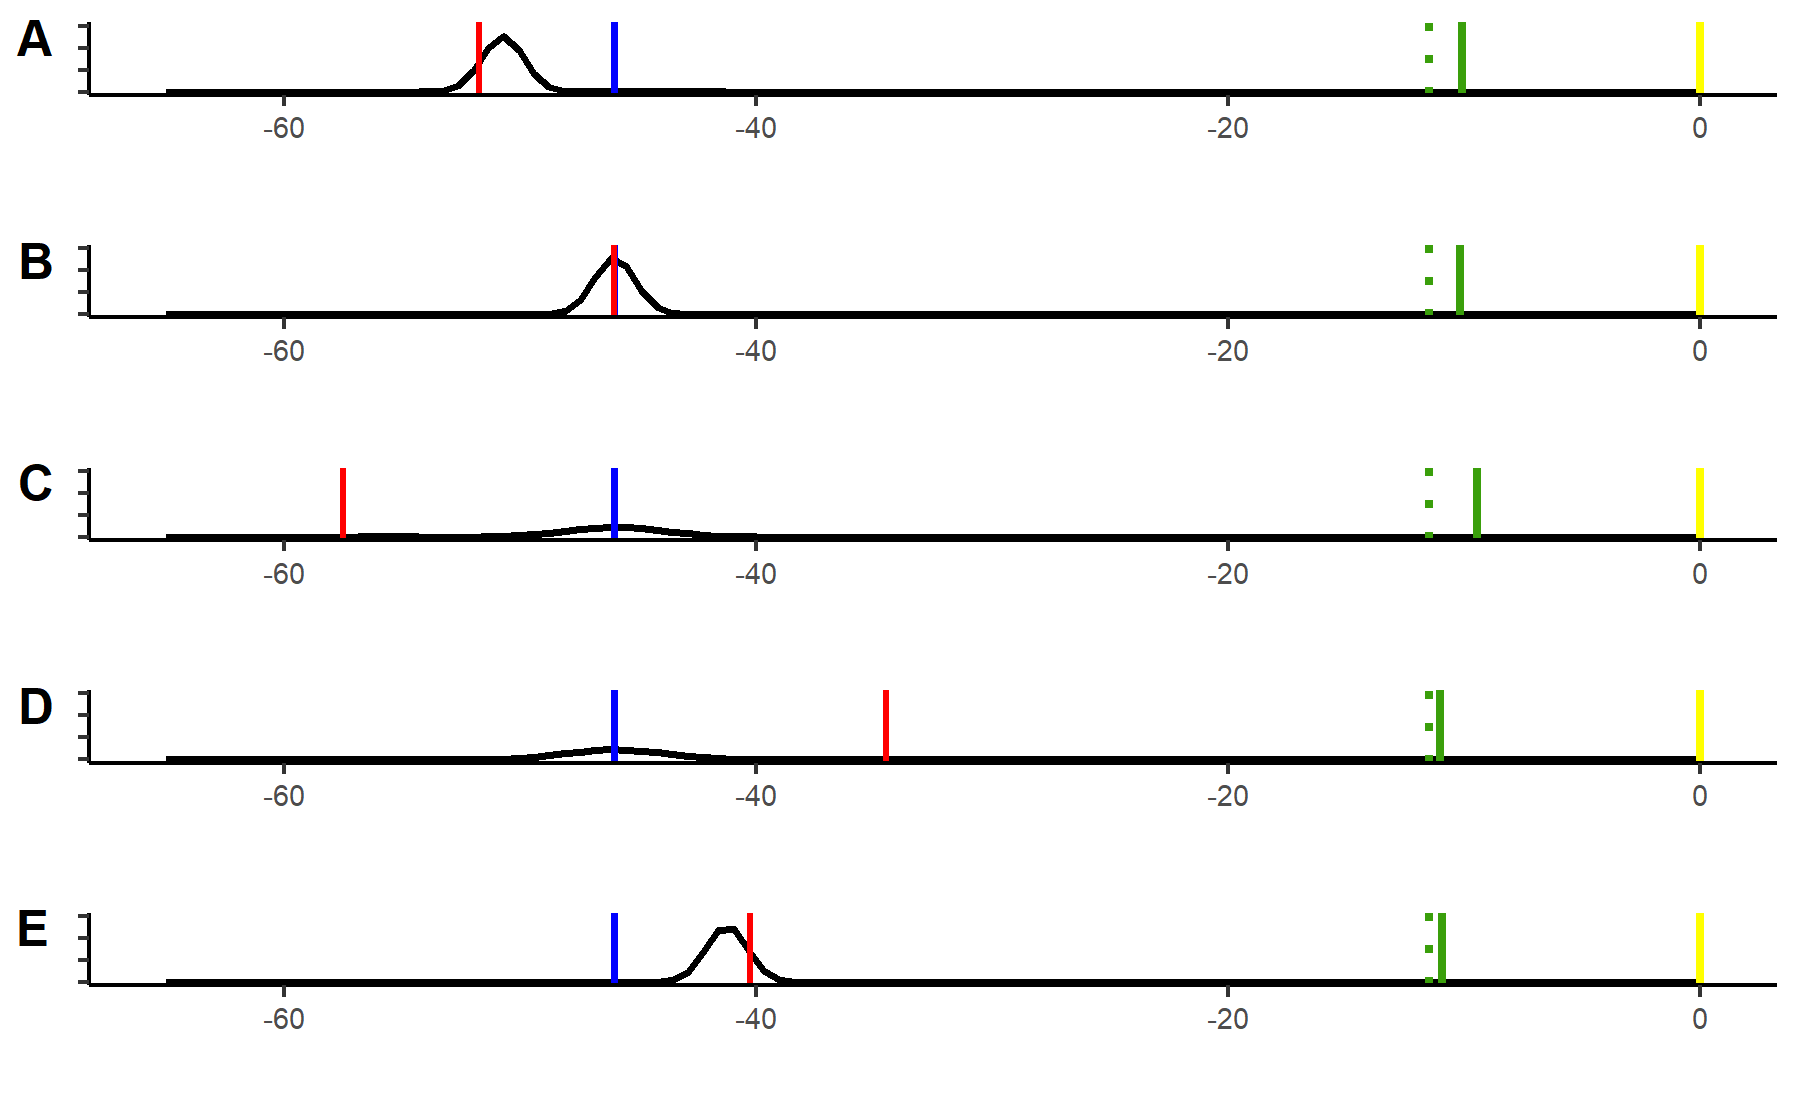
\includegraphics[width=\textwidth, keepaspectratio]{Images/bci-plots/bci_plot34-5.png}
    \caption{Target Location = 11.5 cm}
    \label{}
\end{figure}